\documentclass[pdflatex,compress]{beamer}

%\usetheme[dark,framenumber,totalframenumber]{ElektroITK}
\usetheme[darktitle,framenumber,totalframenumber]{ElektroITK}

\usepackage{lipsum}
\usepackage{graphicx}

\title{FORENSIKA SUARA}
\subtitle{Pengantar Forensika Suara}
\author{Mifta Nur Farid, S.T., M.T.}

\begin{document}

% ----------------------------------------------------------------------------

\maketitle

% ----------------------------------------------------------------------------
\section{Kontrak Perkuliahan}

\subsection{Capaian Pembelajaran Mata Kuliah}

\begin{frame}
	\frametitle{Capaian Pembelajaran Mata Kuliah}
	Mahasiswa mampu menganalisis forensika suara sesuai dengan standard.
\end{frame}

\subsection{Bahan Kajian}

\begin{frame}
	\frametitle{Bahan Kajian}
	\begin{itemize}
		\item Utama:
		\begin{enumerate}
			\item Konsep dasar sinyal suara dan sistem
			\item Sejarah forensika suara
			\item Penanganan barang bukti forensik
			\item Authenticity asssessment
			\item Audio signal enhancement
			\item Forensic interpretation
		\end{enumerate}
		\item Tambahan:
		\begin{enumerate}
			\item Speech Synthesis
			\item Speech Recognition
			\item Speech Emotion Recognition
		\end{enumerate}
	\end{itemize}
\end{frame}

\subsection{Pustaka}
\begin{frame}
	\begin{itemize}
		\frametitle{Pustaka}
		\item Pustaka Utama
		\begin{enumerate}
			\item Maher, R.C., (2018). Principles of Forensic Audio Analysis. New York: Springer.
			\item Wang, D. \& Brown, G. J., (2006). Computational Auditory Scene Analysis. New Jersey: John Wiley \& Sons.
		\end{enumerate}
		\item Pustaka Pendukung
		\begin{enumerate}
			\item Al-Azhar, M. N. (2011). Audio Forensic: Theory And Analysis. Jakarta: Pusat Laboratorium Forensik Polri
			Bidang Fisika Dan Komputer Forensik.
		\end{enumerate}
		\item Dan referensi lainnya yang mendukung perkuliahan ini. Dapat berupa jurnal ilmiah, dsb.
	\end{itemize}
\end{frame}

\begin{frame}
	\frametitle{Jenis dan Bobot Evaluasi}
	\begin{itemize}
		\item Kehadiran
		\item Tugas
		\item Kuis
		\item UTS
		\item UAS
		\item Tugas Besar
	\end{itemize}
\end{frame}

% ----------------------------------------------------------------------------

\section{Pengantar Forensika Suara}

\begin{frame}
	\frametitle{Pengantar}
	\begin{itemize}
		\item Forensika suara (\textit{audio forensics}): salah satu cabang ilmu dari \textit{forensic science}.
		\item \textit{Forensic science}: evaluasi terhadap bukti yang akan digunakan di dalam persidangan atau bagian dari beberapa investigasi formal.
		\item Forensika suara: akusisi, analisis, dan interpretasi terhadap rekaman suara yang merupakan bagian dari investigasi.
		\item Investigasi audio forensik:
		\begin{enumerate}
			\item \textit{Authenticity}.
			\item \textit{Enhancement}.
			\item \textit{Interpretation}.
		\end{enumerate}
	\end{itemize}
\end{frame}

\subsection{Authenticity}

\begin{frame}
	\frametitle{Authenticity}
	\begin{itemize}
		\item Bagian penting dalam investigasi forensik.
		\item Kesimpulan yang diambil oleh investigator dari rekaman suara bergantung pada keadaan di mana rekaman itu dibuat.
		\item Jika ternyata rekaman tersebut diubah/ direkayasa, baik secara sengaja maupun tidak sengaja, sebelum penyelidikan dilakukan, seluruh pemeriksaan akan dipertanyakan.
		\item Apabila terjadi kesalahan, baik disengaja maupun tidak, terkait tempat dan/atau waktu terjadinya perekaman, maka pemeriksaan menjadi tidak relevan.
		\item Examiners $\rightarrow$ mengungkap gangguan yang disengaja, memberikan perlindungan terhadap barang bukti agar terhindar dari perubahan yang tidak disengaja.
	\end{itemize}
\end{frame}

\begin{frame}
	\frametitle{Authenticity}

	\begin{center}
		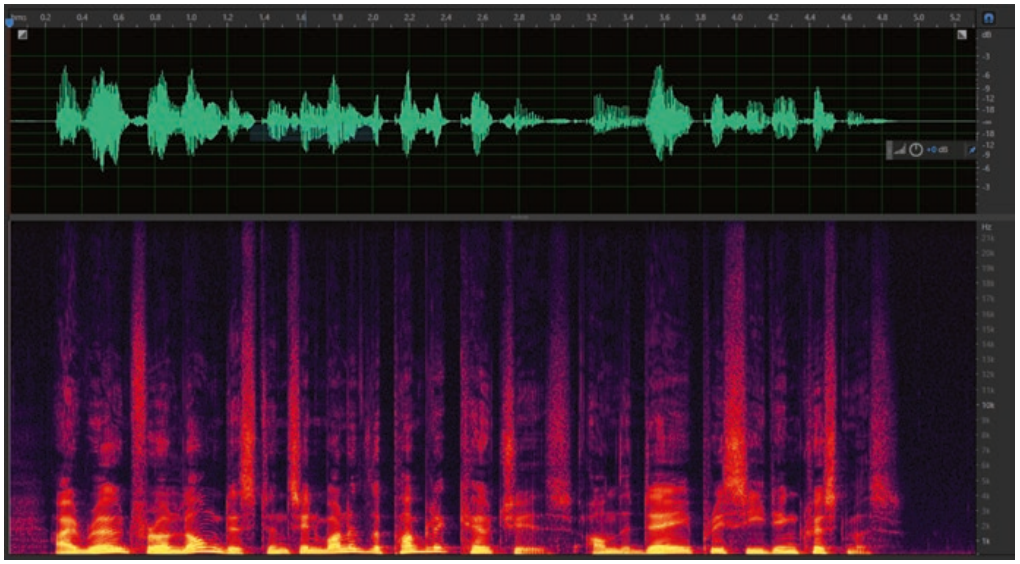
\includegraphics[width=0.8\linewidth]{img/img001}
	\end{center}
	
\end{frame}

\begin{frame}
	\frametitle{Authenticity}
	
	\begin{center}
		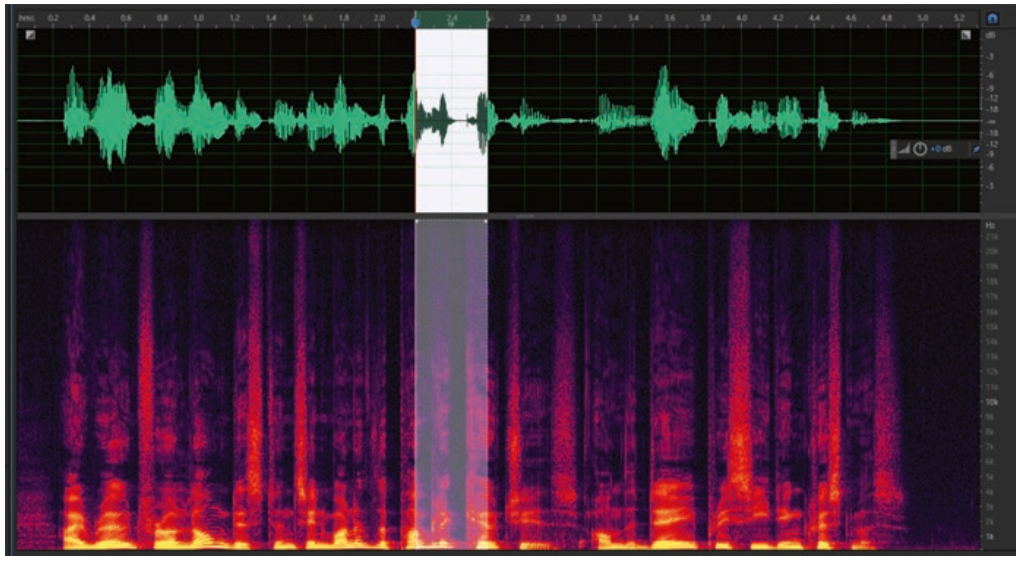
\includegraphics[width=0.8\linewidth]{img/img002}
	\end{center}
	
\end{frame}

\begin{frame}
	\frametitle{Authenticity}
	
	\begin{center}
		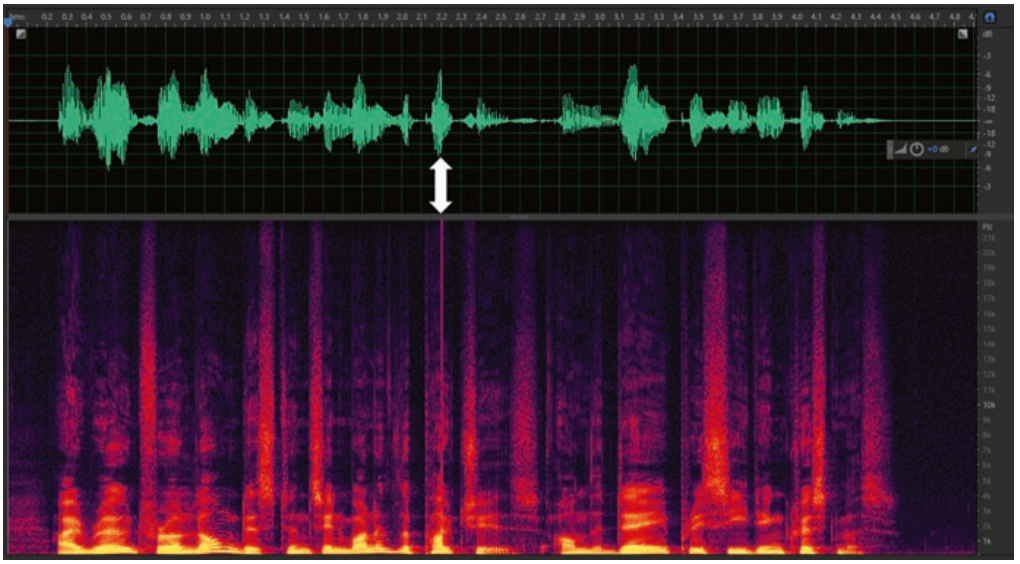
\includegraphics[width=0.8\linewidth]{img/img003}
	\end{center}
	
\end{frame}

\subsection{Audio Enhancement}

\begin{frame}
	\frametitle{Audio Enhancement}
	\begin{itemize}
		\item Kasus yang melibatkan bukti audio forensik sering kali melibatkan permintaan untuk \textit{audio enchancement}.
		\item \textit{Audio enhancement}: Peningkatan kualitas audio.
		\item Audio rekaman biasanya diambil di dalam kondisi akustik yang tidak ideal.
		\begin{itemize}
			\item Posisi mikrofon yang buruk.
			\item \textit{Background noise} yang kuat atau fluktuatif.
			\item Pembicara yang kurang jelas dalam penuturan/pengucapannya.
			\item \textit{Signal of interest}-nya lemah.
		\end{itemize}
		\item Sehingga audio rekaman ini perlu diproses agar informasi yang diinginkan dapat diambil.
	\end{itemize}
\end{frame}

\begin{frame}
	\frametitle{Audio Enhancement}
	
	\begin{center}
		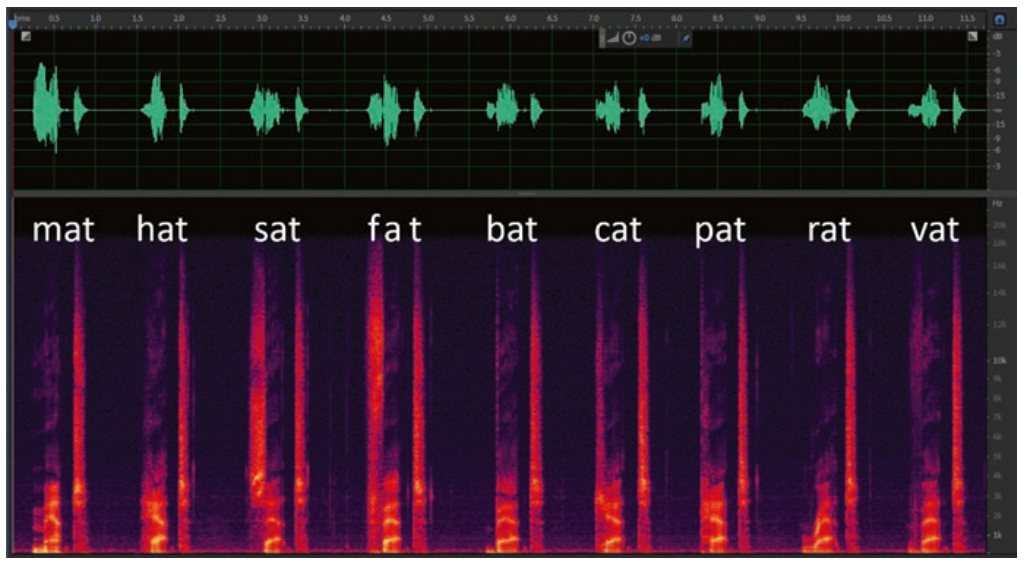
\includegraphics[width=0.8\linewidth]{img/img004}
	\end{center}
	
\end{frame}

\begin{frame}
	\frametitle{Audio Enhancement}
	
	\begin{center}
		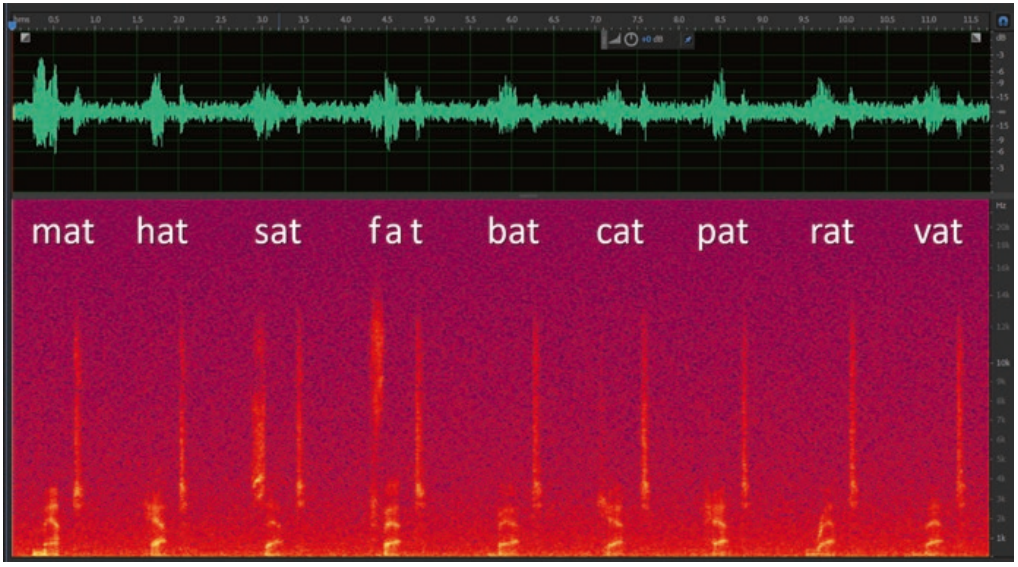
\includegraphics[width=0.8\linewidth]{img/img005}
	\end{center}
	
\end{frame}

\begin{frame}
	\frametitle{Audio Enhancement}
	
	\begin{center}
		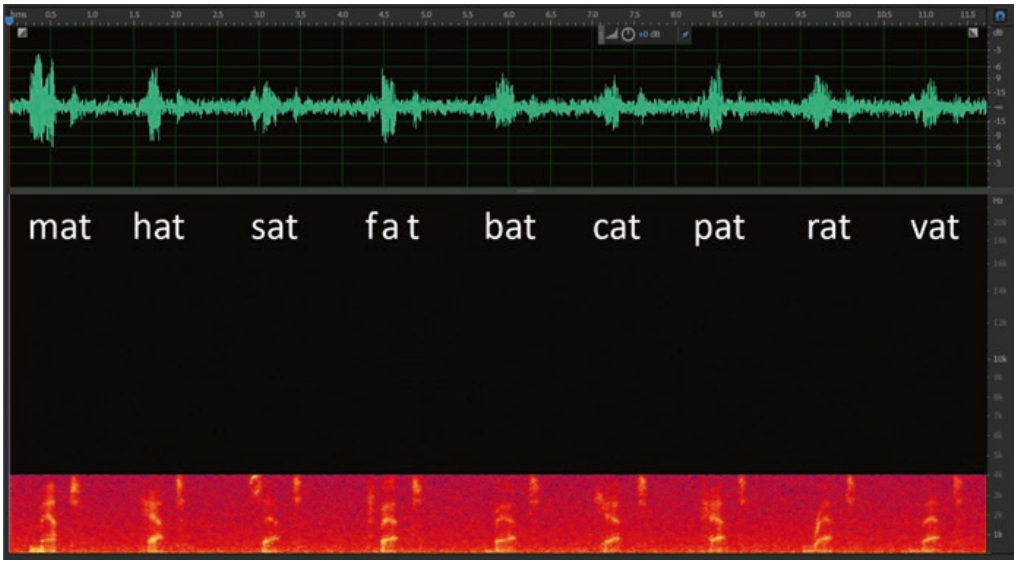
\includegraphics[width=0.8\linewidth]{img/img006}
	\end{center}
	
\end{frame}

\subsection{Interpretation}

\begin{frame}
	\frametitle{Interpretation}
	\begin{itemize}
		\item Melibatkan beberapa hal:
		\begin{enumerate}
			\item \textit{Reconstructing timelines}
			\item \textit{Transcribing dialog}
			\item \text{Identifikasi suara yang tidak diketahui}
		\end{enumerate}
		\item Berdasarkan teori dari investigator: keadaan saat kejahatan terjadi, keterangan saksi, atau bukti fisik lainnya.
	\end{itemize}
\end{frame}

\begin{frame}
	\frametitle{Interpretation}
	
	\begin{center}
		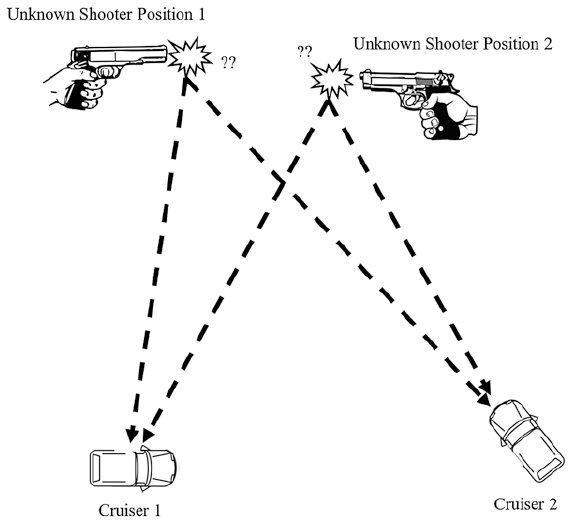
\includegraphics[width=0.6\linewidth]{img/img007}
	\end{center}
	
\end{frame}

\begin{frame}
	\frametitle{Interpretation}
	
	\begin{center}
		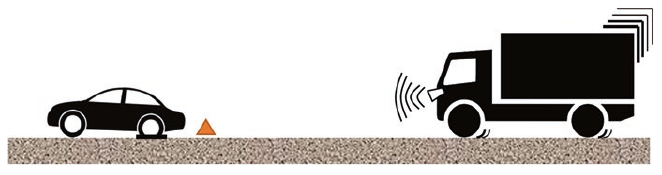
\includegraphics[width=0.8\linewidth]{img/img008}
	\end{center}
	
\end{frame}

\begin{frame}
	\frametitle{Interpretation}
	
	\begin{center}
		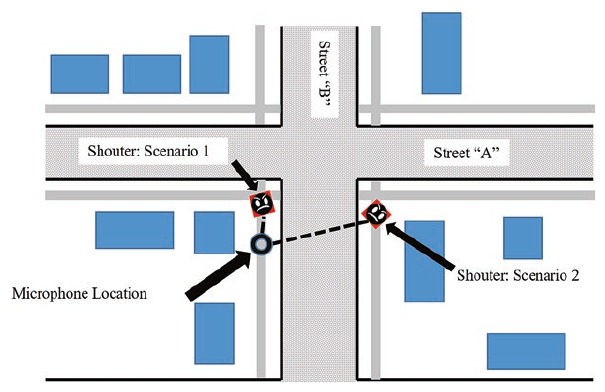
\includegraphics[width=0.8\linewidth]{img/img009}
	\end{center}
	
\end{frame}

\begin{frame}
	\begin{center}
		
\includegraphics[width=\linewidth]{img/img010}
	\end{center}
\end{frame}
% ----------------------------------------------------------------------------

\end{document}
